\documentclass[12pt]{report}
% pre\'ambulo

\usepackage{lmodern}
\usepackage[T1]{fontenc}
\usepackage[spanish,activeacute]{babel}
\usepackage[margin=1in,left=0.7in,right=0.7in,top=1in]{geometry}
\usepackage{mathtools}
\usepackage{bussproofs}
\usepackage{lscape}
\usepackage{resizegather}
\usepackage{verbatim}
\usepackage[utf8]{inputenc}
\usepackage{ amssymb }

\title{Hyperledyer Fabric: Manual de instalación}
\author{René Dávila - Jorge Solano}
\date{ }

\begin{document}
	\maketitle
	% \LaTeX{}.
	\begin{center}
		\textbf{Manual de instalación de Hyperledger Fabric.}
	\end{center}
	
	\textbf{Prerequisitos}\\
	
	\begin{enumerate}
		\item Instalar git: \\https://git-scm.com/downloads.
		\item Instalar cURL: \\https://curl.haxx.se/download.html.
		\item Instalar Docker y Docker Compose (Se requiere la versión 17.06.2-ce o superior): 
		\\https://www.docker.com/get-docker.
		\item Instalar Go: \\https://golang.org/dl/. 
		\item Instalar Node.js y NPM: https://nodejs.org/en/download/.
		\item Instalar Python: https://www.python.org/downloads/.
	\end{enumerate}

	Para construir el escenario de la primera red en Hyperleadger Fabric es necesario, después de instalar los prerequisitos, instalar los ejemplos, binarios e imágenes Docker que se encuentran en https://hyperledger-fabric.readthedocs.io/en/latest/install.html. Para ello hay que inicar Docker Desktop y ejecutar la línea instrucción:
	\begin{center}
		curl -sSL https://bit.ly/2ysbOFE | bash -s
	\end{center}

	La instrucción anterior descarga la carpeta \textit{fabric-samples} en la ubicación actual\\
	
	\begin{figure}[h]
		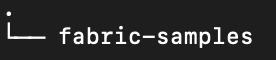
\includegraphics[scale=1]{fabric-samples}
		\centering
	\end{figure}
	
	\newpage
	La fábrica de ejemplos descarga varios proyectos con diferentes escenarios.
	
	\begin{figure}[h]
		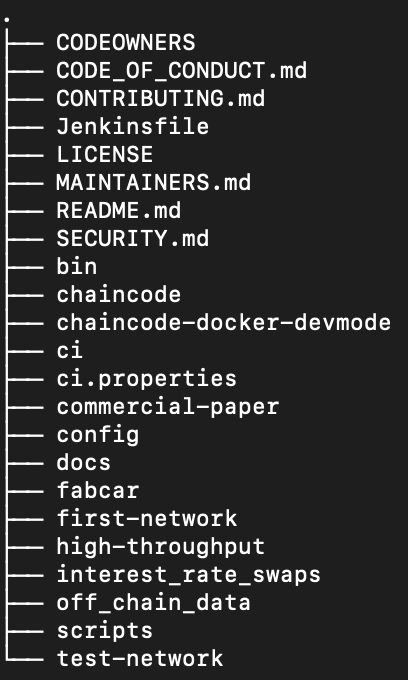
\includegraphics[scale=1]{tree-fabric-samples}
		\centering
	\end{figure}
	
	\newpage
	Para iniciar se recomienda ejecutar el ejemplo test-network, el cual permite ejecutar nodos en la máquina local. Este proyecto también permite probar aplicaciones y contratos inteligentes.
	
	\begin{figure}[h]
		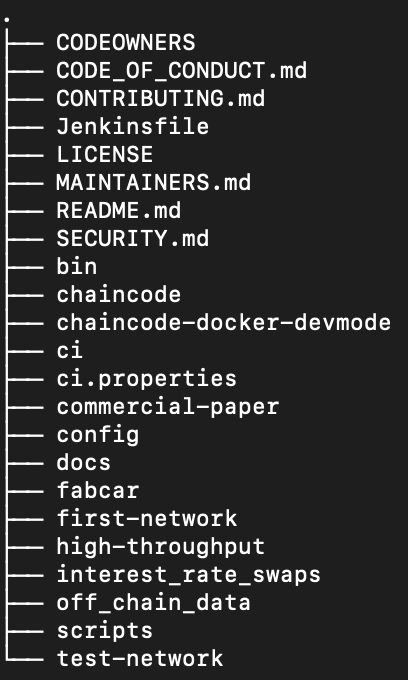
\includegraphics[scale=1]{tree-fabric-samples}
		\centering
	\end{figure}
	
	Si se ejecuta el script byfn.sh (build your first network) sin argumentos, como salida se obtiene una descripción de diversas opciones para ejecutar el ejemplo.\\
	
	\begin{figure}[h]
		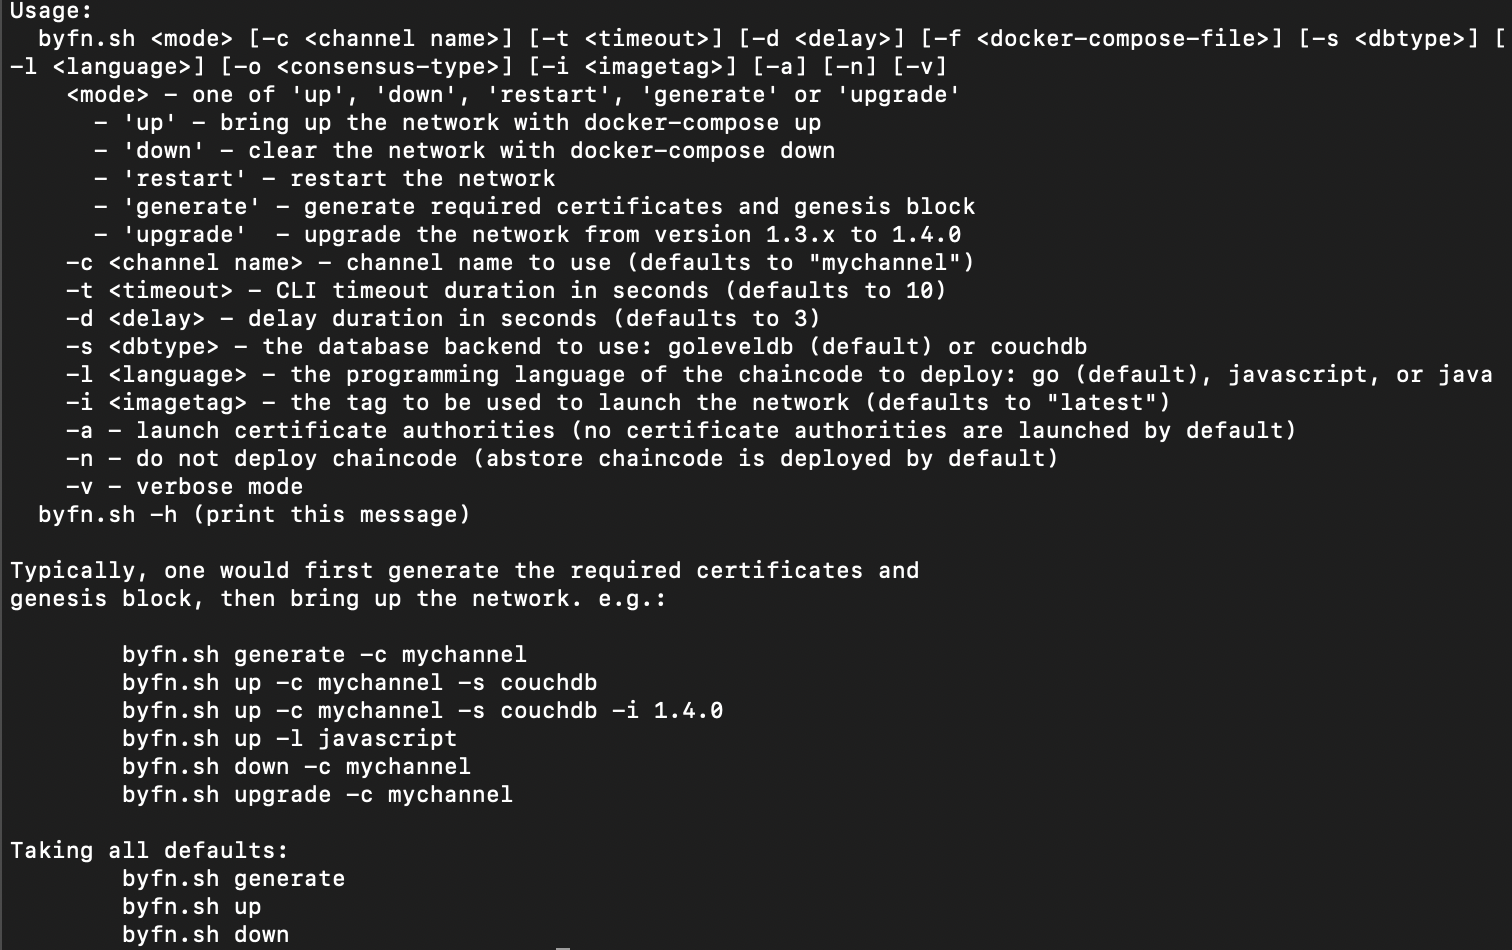
\includegraphics[scale=0.6]{byfn-script}
		\centering
	\end{figure}
	
	\newpage
	Para generar la red \textbf{Artifacts} del ejemplo byfn hay que ejecutar el script con la opción generate (./byfn.sh generate), lo cual genera los certificados de las organizaciones (org1 y org2) y el canal de comunicación (mychannel).\\
	
	\begin{figure}[h]
		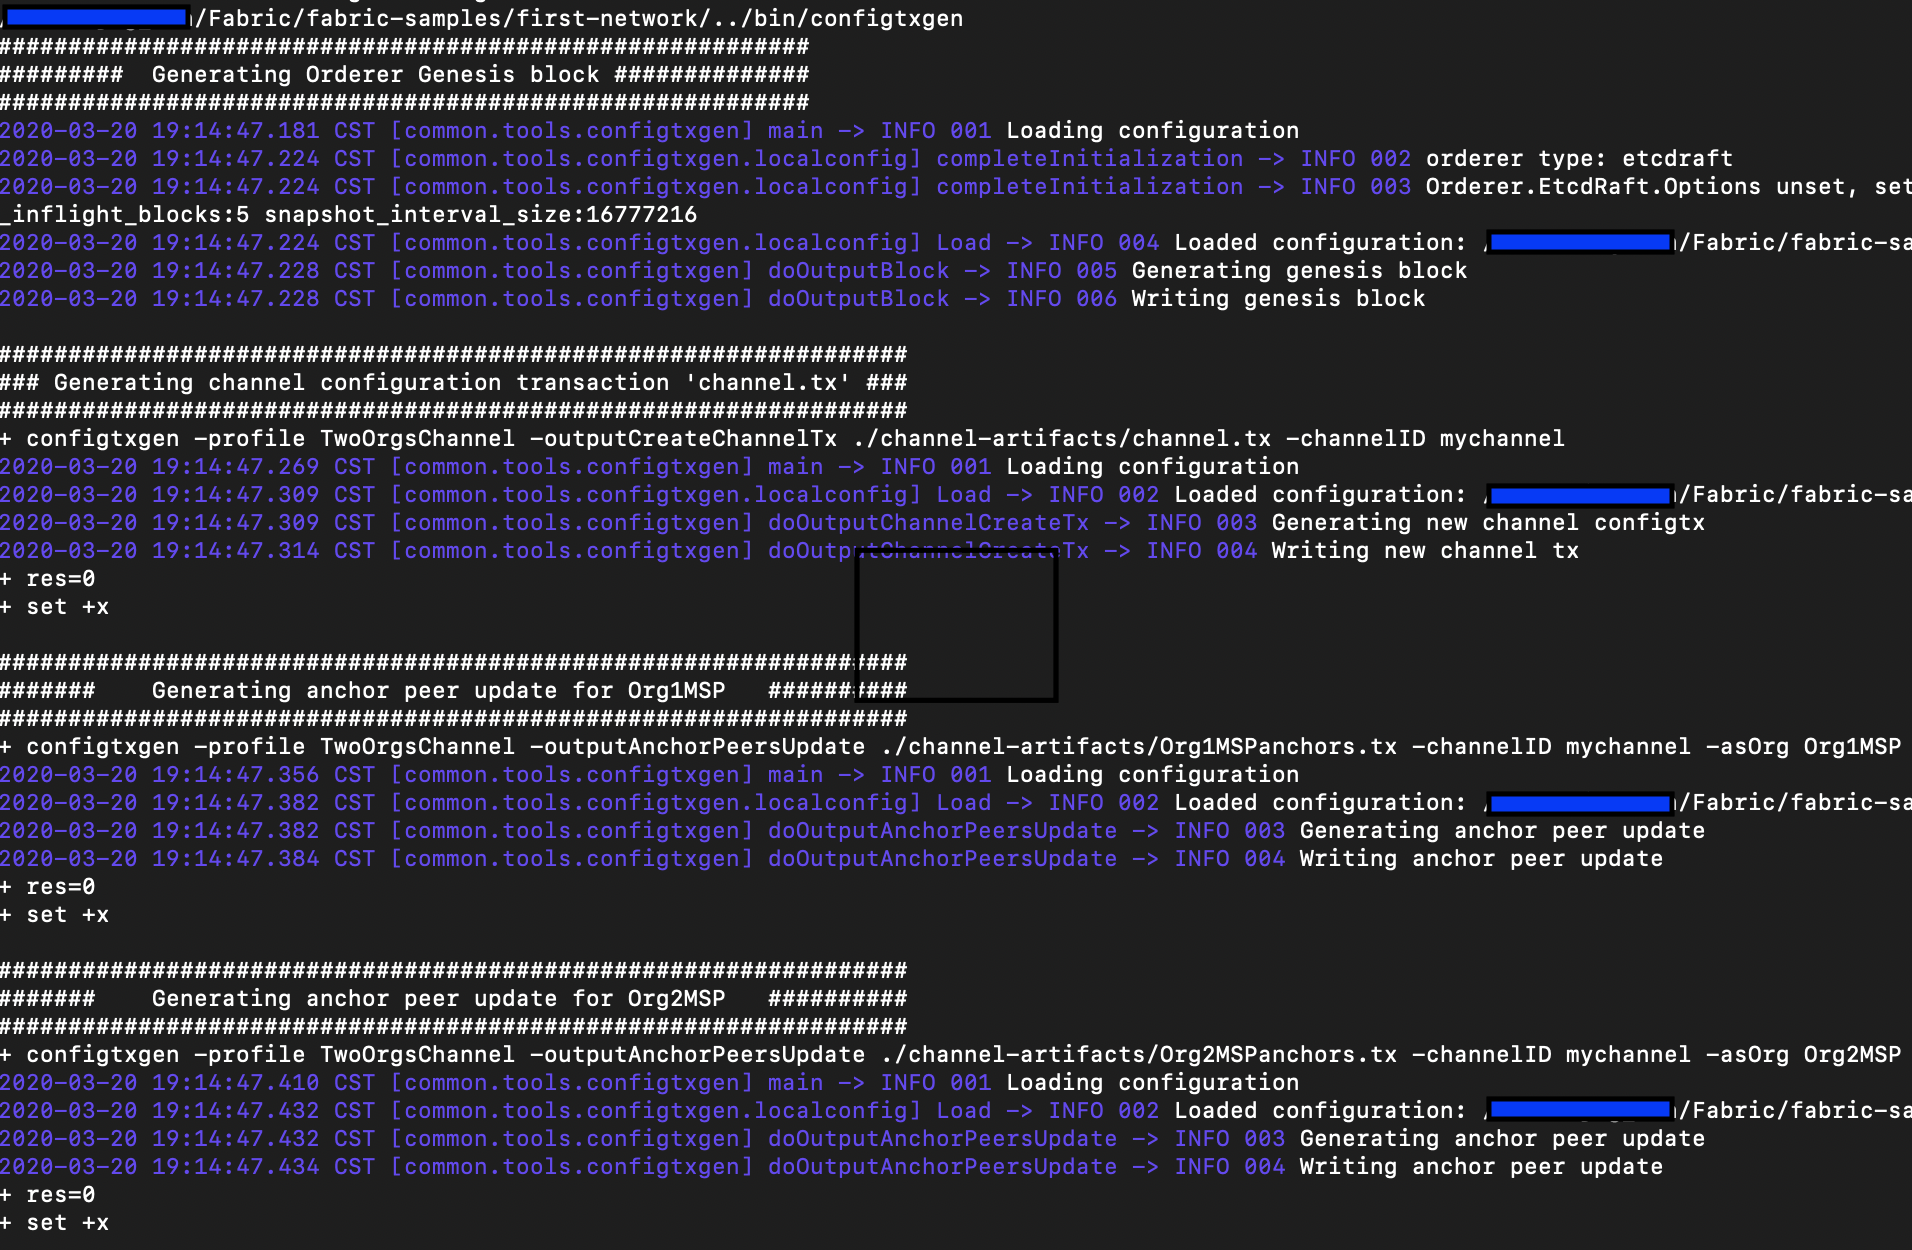
\includegraphics[scale=0.5]{byfn-generate}
		\centering
	\end{figure}
	
	\newpage
	Para levantar la red se ejecuta la instrucción ./byfn.sh up
	
	
	
\end{document}